Customer satisfaction in any software product is highly dependent on the extent to which quality concerns such as performance, security, reliability, and availability~\cite{kruchten2004} are addressed. In practice, a rich set of proven and re-usable architectural solutions in terms of tactics can be used to satisfy each specific quality attribute~\cite{bass:arch12}. Architectural tactics, come in many different shapes and sizes and describe solutions for a wide range of quality concerns~\cite{Hanmer}. For instance, reliability tactics provide solutions for fault mitigation, detection, and recovery. Performance tactics grant solutions for resource contention to optimize response time and throughput. Security tactics provide solutions for authorization, authentication, non-repudiation and other similar factors~\cite{Hanmer}. Such tactics are found prevalently across many software systems~\cite{ICSE2012}.

\subsection{Tactical Spikes}
Archie is built around the fundamental concept of~\emph{Tactical Spikes} which advocates iterative incremental implementation of quality concerns through adoption of individual tactics. For each development cycle, developers focus on a limited number of quality attributes. Tactical Spikes break the development of architecture and satisfaction of quality concerns into small sprints with each focusing on a specific quality attribute and a fine grained design decision which can be implemented independently from other choices. Satisfying quality concerns through Tactical Spikes is not a new idea and has been widely used in incremental design where the architecture emerges through several development cycles.

Although experienced developers are often fully aware of tactics that can be used to implement quality concerns, inexperienced developers tend to ignore the importance of quality attributes or adopt solutions that do not match the context of a problem~\cite{FSE2012}. To integrate agile design thinking into a developer's daily activities, Archie utilizes a knowledge base of architectural tactics and uses this resource to provide suggestions about architectural tactics which can be implemented to address each quality concern. Developers can search the catalogue of quality attributes in Archie and find associated architectural tactics which can be used to implement them. This provides an embedded design resource in the programmer's IDE. 

\subsection{Tool Support}
To implement the idea of Tactical Spikes, we first introduce the fundamental concept of a Tactic Traceability Pattern (TTP)~\cite{Mirakhorli:2011:TAS:1985793.1986014, ICSM11} and then discuss the related functionality. TTP was previously used in maintaining the architecture of safety critical systems. It captures the context that a tactic can be used in, the design knowledge about the tactic, and primary conceptual roles to implement an architectural tactic. For the ~\emph{heartbeat} tactic (Figure~\ref{fig:HB}), the TTP indicates that this tactic can be used to address reliability and availability goals. The primary roles of this tactic include~\emph{emitter},~\emph{receiver}, and~\emph{health monitor}. 

\begin{figure}[tbph]
\centering
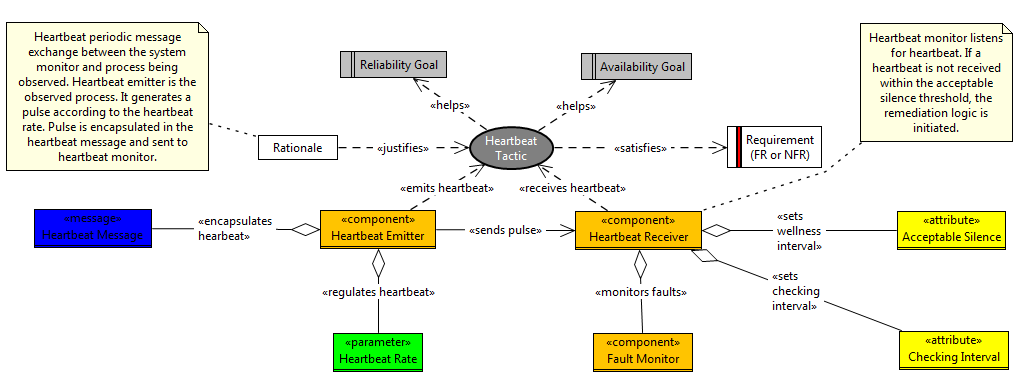
\includegraphics[width=0.9\linewidth]{./HB}
\caption{HeartBeat Traceability Pattern: Helping Developer to Better Adopt and Implement a Tactic}
\label{fig:HB}
\end{figure}


Furthermore, a TTP captures the relationships between these roles i.e. an emitter component sends messages to a receiver, while a health monitor takes actions if the monitored component fails. Lastly, a TTP also captures the underlying rationales for using the tactic which typically come in the form of a description that explains the quality concern being addressed. Each of the provided TTPs are initially populated with a set of default rationales. For example, in the case of heartbeat, these are related to reliability of a critical component. A user can modify rationales and also add references to relevant requirements. Archie ships with a basic set of TTPs including heartbeat, audit, authorization, resource pooling, and scheduler; however a user can utilize Archie's drag-and-drop modeling features to create customized TTPs.


The idea of Tactical Spikes are supported by TTP artifacts. Whenever developers want to implement a quality concern, they can look at the catalogue of TTPs in Archie and find the appropriate tactics which can be used to address their interested quality requirements. Furthermore, they would get an initial idea about which conceptual roles are involved when implementing the tactic. TTPs are modifiable artifacts (models), the developers can revise a TTP and document their micro design using basic UML modeling notations, they can also connect the tactical roles in the TTP to the source code. This can be done simply by selecting a segment of code and using mouse clicks to map it to either the entire TTP or to a specific role. Once the TTP is connected to the source code, it can provide a visual framework for communicating underlying architectural knowledge with other developers.
